\subsection{UC-26}
\label{subsec:UC-26}

\begin{figure}[H]
    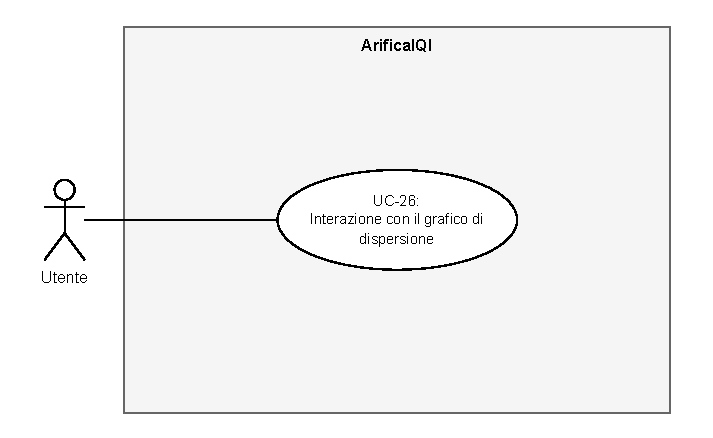
\includegraphics{Sezioni/UseCase/Immagini/UC-26.pdf}
    \caption{Diagramma UC-26.}
\end{figure}

\begin{usecase}{UC-26}{Interazione con il grafico di dispersione}

    \req{} 

    \pre{
        \item Il sistema è attivo e funzionante
        \item L'utente dispone del grafico di dispersione prodotto nella visualizzazione dei risultati del test
    }

    \post{
        \item Viene evidenziato il risultato relativo al punto del grafico di dispersione coinvolto nell'interazione
    }
    
    \actor{Utente}

    \subactors{LLM}

    \trigger{L'utente ha la necessità di visualizzare un preciso risultato}
    
    \inc{}

    \base{}

    \scenario{
        \item L'utente interagisce con un punto del grafico di dispersione
        
        \item Viene evidenziato l'elemento della lista dei risultati corrispondente al punto coinvolto nell'interazione
    }

\end{usecase}